\documentclass[a4paper,10pt]{article}

\usepackage[margin=1in]{geometry} 	% Setea el margen manualmente, todos iguales.
\usepackage[spanish]{babel} 		% {Con estos dos anda
\usepackage[utf8]{inputenc} 		% todo lo que es tildes y ñ}
\usepackage{fancyhdr} 			%{Estos dos son para
\usepackage{ulem}
\pagestyle{fancyplain} 			% el header copado}
\usepackage{color}			% Con esto puedo hacer la matufia de poner en color blanco un texto para engañar al formato
\usepackage{graphicx}	% Para insertar gráficos
\usepackage{array}			% Para usar arrays
\usepackage{hyperref}		% Para que tenga links el índice
\usepackage{lscape}         % Para apaisar figuras
\usepackage{ textcomp }
\usepackage{ulem}

%\usepackage{datetime}	% Para agregar automáticamente fecha/hora de compilación y otras cosas

\lhead{Bases de Datos} 	% {Con esto se usa el header copado. También está \chead para
\rhead{TP1} 	% el centro y comandos para el pie de página, buscar fancyhdr}
\renewcommand{\footrulewidth}{0.4pt}
\lfoot{Facultad de Ciencias Exactas y Naturales}
\rfoot{Universidad de Buenos Aires}
%\rfoot{\textit{}}
\usepackage{amsfonts}	% para simbolos de reales, naturales, etc. se usa \mathbb{•} y la letra
\usepackage{amsmath}	% para \implies
%\usepackage{algorithm}
%\usepackage{algorithmic}
\usepackage{caratula}
\usepackage{pdfpages}

%%%%%%%%%%%%%%%%%%%%%%%%%%%%%%%%%%%%%
%      COMANDOS ÚTILES USADOS       %
%%%%%%%%%%%%%%%%%%%%%%%%%%%%%%%%%%%%%

% \section{title} 		Te hace un título ``importante'' en negrita, numerado. También está \subsection{title} y \subsubsection{title}.
% \begin{itemize}		Te hace viñetas.
%	\item esto es un item	Cambiar itemize por enumerate te hace una numeración.
% \end{itemize}

% \textbf{text} 		Te hace el texto en negrita (bold).
% \underline{text}		Te subraya el texto.

% \textsuperscript{text}	Te hace ``superindices'' con texto. En teoría subscript debería funcionar, pero se puede usar guion bajo entre llaves
% 				y signos peso para hacerlo como alternativa. Sino buscar.

% \begin{tabular}{cols} 	Es para hacer tablas. Se pone una c por cada columna deseada dentro de cols (si es que se desea centrada, l para justificar a 
%	a & b & c		izquierda, r a la derecha). Si se separa por espacios la tabla no tendrá líneas divisorias. Si se separa por | en lugar de 
% \end{tabular}			espacios, aparecerá una línea. Con || dos, y así. Luego para los elementos de las filas se escriben y se separan con ampersand (&).
%				Finalmente, para las líneas horizontales, se usa \hline para una linea en toda la tabla y \cline{i - j} te hace la linea desde
%				la celda i hasta la j, arrancando en 1.
%				Si en la columna se pone p(width) podés escribir un párrafo en la celda. Para hacer un enter con \\ no funciona porque te hace un
%				enter en la fila. Para eso se usa el comando \newline.
  
% \textcolor{color predefinido en palabras}{text}

%%%%%%%%%%%%%%%%%%%%%%%%%%%%%%%%%%%%%
%    FIN COMANDOS ÚTILES USADOS     %
%%%%%%%%%%%%%%%%%%%%%%%%%%%%%%%%%%%%%

\newcommand{\Gather}[1]{\begin{gather*}#1\end{gather*}}
%\newcommand{\Def}[1]{\textbf{Definición: }#1}
%\newcommand{\Prop}[1]{\textbf{Propiedad: }#1}
%\newcommand{\Teo}[1]{\textbf{Teorema: }#1}
\newcommand{\Obs}[1]{\textbf{Observación: }#1}
%\newcommand{\Amat}{A \in \mathbb{R}^{n\textnormal{x}n}}
\newcommand{\filtro}[1]{\textbf{\textit{#1}}}
\renewcommand{\labelenumii}{\theenumii}
\renewcommand{\theenumii}{\theenumi.\arabic{enumii}.}

\begin{document}

%%%%%%%%%%%%%%%%%%%%%%%%%%%
%			INICIO DE CARÁTULA			%
%%%%%%%%%%%%%%%%%%%%%%%%%%%

%% **************************************************************************
%
%  Package 'caratula', version 0.2 (para componer caratulas de TPs del DC).
%
%  En caso de dudas, problemas o sugerencias sobre este package escribir a
%  Nico Rosner (nrosner arroba dc.uba.ar).
%
% **************************************************************************



% ----- Informacion sobre el package para el sistema -----------------------

\NeedsTeXFormat{LaTeX2e}
\ProvidesPackage{caratula}[2003/4/13 v0.1 Para componer caratulas de TPs del DC]


% ----- Imprimir un mensajito al procesar un .tex que use este package -----

\typeout{Cargando package 'caratula' v0.2 (21/4/2003)}


% ----- Algunas variables --------------------------------------------------

\let\Materia\relax
\let\Submateria\relax
\let\Titulo\relax
\let\Subtitulo\relax
\let\Grupo\relax


% ----- Comandos para que el usuario defina las variables ------------------

\def\materia#1{\def\Materia{#1}}
\def\submateria#1{\def\Submateria{#1}}
\def\titulo#1{\def\Titulo{#1}}
\def\subtitulo#1{\def\Subtitulo{#1}}
\def\grupo#1{\def\Grupo{#1}}


% ----- Token list para los integrantes ------------------------------------

\newtoks\intlist\intlist={}


% ----- Comando para que el usuario agregue integrantes

\def\integrante#1#2#3{\intlist=\expandafter{\the\intlist
	\rule{0pt}{1.2em}#1&#2&\tt #3\\[0.2em]}}


% ----- Macro para generar la tabla de integrantes -------------------------

\def\tablaints{%
	\begin{tabular}{|l@{\hspace{4ex}}c@{\hspace{4ex}}l|}
		\hline
		\rule{0pt}{1.2em}Integrante & LU & Correo electr\'onico\\[0.2em]
		\hline
		\the\intlist
		\hline
	\end{tabular}}


% ----- Codigo para manejo de errores --------------------------------------

\def\se{\let\ifsetuperror\iftrue}
\def\ifsetuperror{%
	\let\ifsetuperror\iffalse
	\ifx\Materia\relax\se\errhelp={Te olvidaste de proveer una \materia{}.}\fi
	\ifx\Titulo\relax\se\errhelp={Te olvidaste de proveer un \titulo{}.}\fi
	\edef\mlist{\the\intlist}\ifx\mlist\empty\se%
	\errhelp={Tenes que proveer al menos un \integrante{nombre}{lu}{email}.}\fi
	\expandafter\ifsetuperror}


% ----- Reemplazamos el comando \maketitle de LaTeX con el nuestro ---------

\def\maketitle{%
	\ifsetuperror\errmessage{Faltan datos de la caratula! Ingresar 'h' para mas informacion.}\fi
	\thispagestyle{empty}
	\begin{center}
	\vspace*{\stretch{2}}
	{\LARGE\textbf{\Materia}}\\[1em]
	\ifx\Submateria\relax\else{\Large \Submateria}\\[0.5em]\fi
	\par\vspace{\stretch{1}}
	{\large Departamento de Computaci\'on}\\[0.5em]
	{\large Facultad de Ciencias Exactas y Naturales}\\[0.5em]
	{\large Universidad de Buenos Aires}
	\par\vspace{\stretch{3}}
	{\Large \textbf{\Titulo}}\\[0.8em]
	{\Large \Subtitulo}
	\par\vspace{\stretch{3}}
	\ifx\Grupo\relax\else\textbf{\Grupo}\par\bigskip\fi
	\tablaints
	\end{center}
	\vspace*{\stretch{3}}
	\newpage}

\materia{Bases de Datos}
\submateria{Segundo Cuatrimestre de 2014}
\titulo{Trabajo Práctico }

\grupo{}
\integrante{Martinez Suñe, Agustín}{630/11}{aemartinez@dc.uba.ar}
\integrante{Iglesias, Axel}{79/10}{axeligl@gmail.com}
\integrante{Lascano, Nahuel}{476/11}{laski.nahuel@gmail.com}
\integrante{Artuso, Pablo}{282/11}{artusopablo@gmail.com}

\begin{titlepage}
\maketitle
\thispagestyle{empty}
\end{titlepage} 

%%%%%%%%%%%%%%%%%%%%%%%%%%%
%				FIN DE CARÁTULA			%
%%%%%%%%%%%%%%%%%%%%%%%%%%%

\tableofcontents
%\clearpage

%%%%%%%%%%%%%%%%%%%%%%%%%%%
%					DESARROLLO				%
%%%%%%%%%%%%%%%%%%%%%%%%%%%

\section{Introducción}
Con el avance de la tecnología y la capacidad de almacenamiento, las bases de datos tienden a almacenar cada vez más información. En un principio parece una ventaja, sin embargo, se puede inferir fácilmente que un almacenamiento masivo puede ocasionar problemas a la hora de realizar búsquedas. Mientras más grande es el espacio de búsqueda, mayor será el tiempo a invertir para lograr el objetivo.

El \textbf{optimizador de consultas}, componente clave del motor de base de datos, es el que combate el problema del tiempo antes mencionado. Su misión es, como bien explica su propio nombre, tratar de optimizar la forma de realizar la consulta con el fin de obtener la respuesta lo más rápido posible. Entre muchas otras cosas, el componente hace un fuerte uso de \textbf{estimadores} para poder llevar a cabo la optimización. Un \textbf{estimador} es un componente que brinda información aproximada de la cantidad de elementos que cumplen cierta condición (también llamada \textbf{selectividad}) comparativa contra una constante dada. Por lo tanto, el optimizador intentará reescribir la consulta de distintas maneras (manteniendo su valor semántico) y a través de distintas estimaciones, tomar una desición de cuál será la forma más eficiente de realizar la consulta. Si bien la precisión de la estimación debe ser lo más ajustada posible tiene también importancia la velocidad con la que se realiza, dado que este procedimiento se repetirá por cada consulta a la base. Es por esto que el estimador debe estar organizado de modo tal que pueda resolver rápidamente las consultas pedidas, quizás a cambio de tomarse más tiempo a la hora de inicializarlo o reiniciarlo. Del mismo modo, la elección del estimador afecta fuertemente la precisión de los resultados, por lo cual el conocimiento sobre la información específica de los elementos (distribución, dispersión, densidad, etc.) juega un papel determinante a la hora de la elección del estimador.

En el presente trabajo, detallamos tres implementaciones distintas de estimadores, mostrando sus diferentes comportamientos frente a distintas distribuciones, comparándolos y extrayendo conclusiones.
\section{Diagrama Entidad Relación}
\subsection{Diseño}
A continuación se observa el modelo completo que diseñamos como solución al problema planteado.

\begin{figure}[h!]
  \centering
  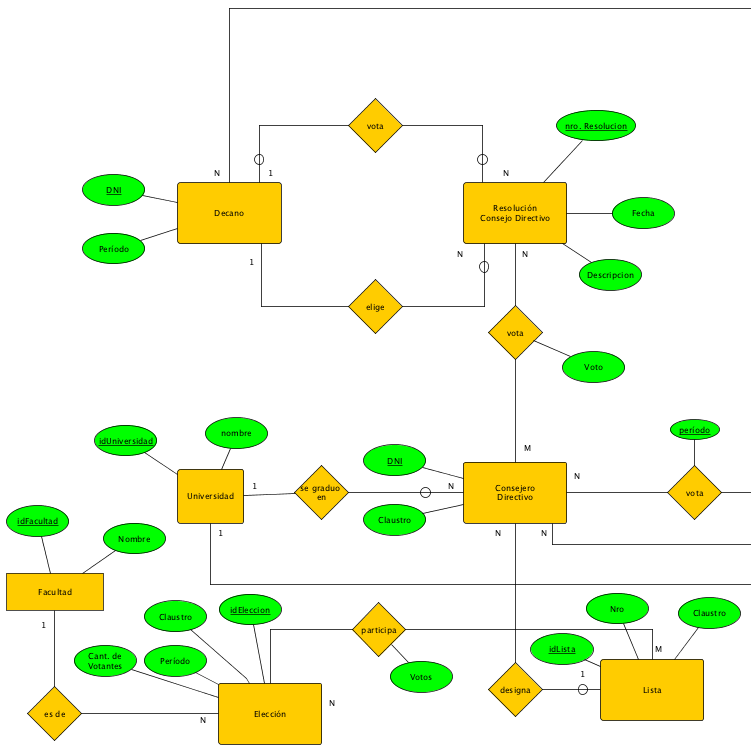
\includegraphics[width=1\textwidth]{./images/der1}
  \caption{Primera parte del Diagrama Entidad Relación}
  \label{fig:clases4}
\end{figure}

\begin{figure}[h!]
  \centering
  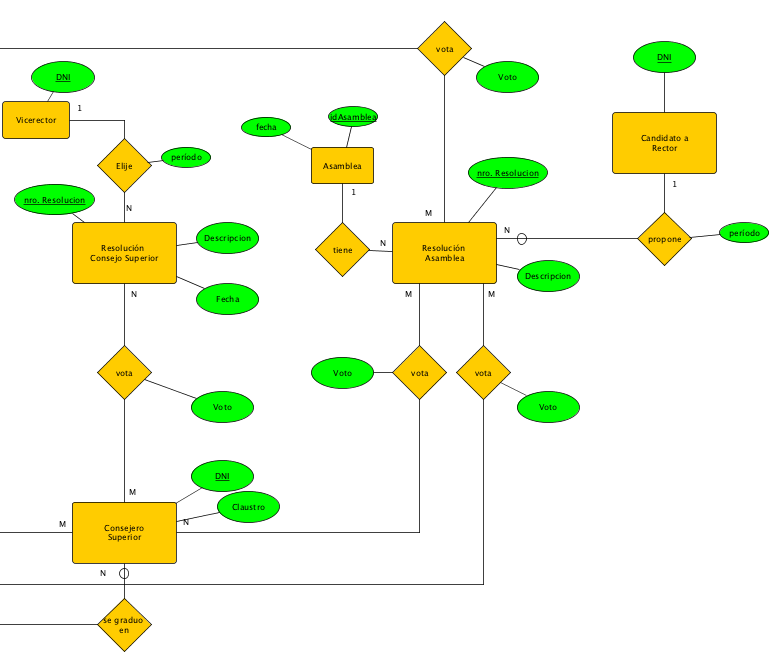
\includegraphics[width=1\textwidth]{./images/der2}
  \caption{Segunda parte del Diagrama Entidad Relación}
  \label{fig:clases4}
\end{figure}
\newpage
\subsection{Consideraciones}
Estas son algunas asunciones que hicimos con el fin de simplificar el modelo.

\begin{itemize}
\item  No es necesario tener la información de todo el padrón de cada claustro, ya que la votación de consejeros directivos es secreta.
\item Al no modelar los integrantes de cada claustro no modelamos las condiciones que deben cumplir los candidatos a los diferentes cargos. Asumimos que las personas que estan en cada una de esas tablas cumplen las condiciones. Esto es:
	\begin{itemize}
    \item Pueden ser candidatos por el claustro de profesores los profesores titulares plenarios, titulares asociados, profesores consultos y eméritos de cualquier Facultad de la UBA.
    \item Pueden ser candidatos por el claustro de graduados quienes hayan obtenido su diploma por la UBA (siempre y cuando no sean profesores) o los graduados de otras universidades nacionales con iguales títulos si acreditan actividad profesional de al menos dos años en la UBA.
    \item Pueden ser candidatos por el claustro de estudiantes cualquier alumno regular de una carrera que tengan al menos un año de antiguedad en la inscripción.
    \item Para ser rector hace falta ser ciudadano argentino, tener 30 años o más y ser o haber sido profesor de alguna Universidad Nacional.
    \end{itemize}
\item Las resoluciones rechazadas también son registradas: para cada par resolución/consejero, el atributo de la relación ''vota'' (llamado ''voto'') indica si el mismo fue positivo o negativo. Contabilizando los votos positivos sobre el total se puede saber si la resolución fue aprobada o no.
\item Por el mismo motivo, no modelamos explícitamente cuando un candidato a decano/rector es efectivamente elegido, sino que esta informacion se deduce de la cantidad de votos que recibió cada candidato. Esto es porque las elecciones se realizan por medio de resoluciones: cada consejero vota una resolución que promueve a su candidato como decano/rector. De esas resoluciones, la que resulta finalmente aprobada 'elige'' al decano/rector ganador. De esta manera podemos saber a qué candidato vota cada consejero, y también detectar empates o falta de quórum (si ninguna resolución de cierta fecha terminó eligiendo un candidato).
\end{itemize}

\subsection{Aclaraciones}
Estas son algunas aclaraciones a tener en cuenta sobre cosas que podrían no quedar claras en el DER.
\begin{itemize}
\item En nuestro afán de evitar la redundancia, podría parecer que hay información faltante (por ejemplo, de qué facultad es cierto Consejero Directivo), sin embargo nos preocupamos mucho por que toda la información necesaria sea accesible de algún modo (el Consejero es designado por una Lista que participa en una Elección que pertenece a una Facultad).
\item No incluimos en el modelo la totalidad de atributos de las entidades que podrían resultar interesantes, porque consideramos que esa información puede cambiar rápidamente y el enunciado no especifica cuáles son. Naturalmente entendemos que quien opere la base va a querer guardar el apellido de los candidatos, la dirección de las Facultades, el texto completo de las resoluciones, etc., pero por economía de espacio y para no sobre-especificar decidimos dejar la elección de los atributos a una etapa posterior. Sí incluimos, como puede observarse, todos los atributos necesarios para obtener la información necesaria para resolver las consultas especificadas.
\end{itemize}

\subsection{Restricciones}
Para que el modelo cumpla con lo estipulado en el estatuto, se deben tener en cuenta las siguientes restricciones extras:

\begin{itemize}
\item Una misma lista no puede estar en dos elecciones de distintas facultades.
\item Todas las resoluciones de Consejo Directivo son votadas por consejeros de la misma facultad.
\item Los consejeros directivos solo votan consejeros superiores de su propio claustro.
\item 'M' es 5 en la relación de votación de Consejero Directivo y Consejero Superior
\item Las resoluciones de Consejo Directivo son votadas por 4 Consejeros estudiantiles, 4 graduados y 8 profesores, correspondientes a la facultad y período de la resolución.
\item La composición del Consejo Directivo cumple lo especificado en el estatuto (por ejemplo para estudiantes, 3 para la mayoría y 1 para la primer minoría si llega al 20\% de los votos).
\item Las resoluciones que forman parte de la relación ''vota'' con un decano/rector son las que proponen a un candidato como decano/rector. Las que además forman parte de la relación ''elige'' son las ganadoras de esa elección.
\item Ningún consejero puede ser representante por dos claustros en el mismo período.
\end{itemize}

\section{Modelo Relacional}
Este es el MR correspondiente a DER presentado anteriormente. En él se pueden ver las distintas tablas necesarias para realizar la implementación.


\noindent \textbf{Decano}(\underline{DNI}, Periodo) \\
\textbf{ResolucionConsejoDirectivo}(\underline{nroResolucion}, Fecha, \dashuline{idDecanoQueVota}, \\\dashuline{idDecanoElegido})\\
\textbf{ResolucionConsejoSuperior}(\underline{nroResolucion}, Fecha)\\
\textbf{Asamblea}(\underline{idAsamblea}, fecha)\\
\textbf{ResolucionAsamblea}(\underline{nroResolucion}, \dashuline{idAsamblea, idCandidatoRector, idCandidatoVicerrector})\\
\textbf{CandidatoARector}(\underline{DNI}, periodo)\\
\textbf{Universidad}(\underline{idUniversidad}, nombre)\\
\textbf{ConsejeroDirectivo}(\underline{DNI}, Claustro, \dashuline{idUniversidad, idLista})\\
\textbf{ConsejeroSuperior}(\underline{DNI}, Claustro, \dashuline{idUniversidad})\\
\textbf{Lista}(\underline{idLista}, Nro, Claustro)\\
\textbf{Facultad}(\underline{idFacultad}, Nombre)\\
\textbf{Eleccion}(\underline{idEleccion}, Periodo, CantDeVotantes, \dashuline{idFacultad})\\
\textbf{CandidatoAVicerrector}(\underline{DNI})\\
\textbf{VotaDecanoAsamblea}(\underline{idDecano, nroResolucion}, voto)\\
\textbf{VotaSuperiorAsamblea}(\underline{DNI}, voto)\\
\textbf{VotaDirectivoAsamblea}(\underline{DNI}, voto)\\
\textbf{VotaResolucionDirectivo}(\underline{DNI, nroResolucion}, voto)\\
\textbf{VotaResolucionSuperior}(\underline{DNI, nroResolucion}, voto)\\
\textbf{VotaDirectivoSuperior}(\underline{DNI\_Directivo, DNI\_Superior, periodo})\\
\textbf{Participa}(\underline{idLista, idEleccion})\\


\section{Consultas}

En esta sección vamos a explicar en castellano cómo se pueden resolver las consultas pedidas en el enunciado.

\begin{itemize}
\item \textbf{La cantidad de elecciones de Rector que requirieron al menos 3 sesiones de votación para llegar a un resultado satisfactorio}

Nuestro modelo considera la tabla de candidatos a Rector donde se registra los distintos candidatos. Cada uno de estos candidatos está relacionado con su resolución de asamblea correspondiente, considerando el período al cual se postula. Al contabilizar los votos de cada uno de los asambleístas se logra identificar aquellos cuya cantidad de votos no alcanza para asumir.
Al tener como atributo relacional el período podemos considerar aquellos períodos para los cuales fue necesario variadas instancias de votación: si resoluciones de asambleas distintas proponen un rector para el mismo período quiere decir que fueron necesarias varias elecciones para elegirlo.

\item \textbf{Los nombres de las 5 personas con mayor cantidad de participaciones en Asambleas Universitarias}

Al tener el DNI como atributo de los distintos cargos nominales de los órganos de cogobierno es sencillo buscar aquellas personas que fueron parte de asambleas universitarias, no importa cual haya sido su cargo, viendo las resoluciones de las asambleas y votaciones en las cuales participaron.

\item \textbf{Porcentaje  histórico  de  representantes  del  Claustro  de  Graduados  de  la UBA que se graduaron en otra universidad nacional}

Para esto, guardamos para aquellos consejeros (Directivos o Superiores) que sean graduados la información de en qué Universidad se graduaron. De este modo, podemos calcular el porcentaje de graduados que se graduaron en otra universidad nacional. Se deberá tener en cuenta que sean personas distintas (DNI distinto) ya que una persona puede ser Consejero varios años y en varios cuerpos (por ejemplo ser primero Directivo y luego Superior).

\item \textbf{Resolución de algunas de las restricciones del enunciado utilizando triggers}
Podemos hacer que el motor cree automáticamente las relaciones ''elige'' cuando un candidato a Decano/Rector tiene suficientes votos positivos en la Resolución correspondiente a su designación. Solo hace falta implementar las reglas para la elección de cada uno de ellos:
  \begin{itemize}
  \item El Decano requiere por lo menos 9 de 16 votos.
  \item El Rector requiere la mitad más uno de los votos, salvo que sea la tercera vez que se reúne la asamblea para este período, en cuyo caso solo le hace falta superar a todos los demás candidatos.
  \end{itemize}
\end{itemize}









\end{document}
